\chapter{Research Description}
\label{sec:researchdesc}    %--note: labels help you with hyperlink editing (using your IDE)

This chapter contains an introduction to the definition and common uses of augmented reality, software applications that involve the generation of the 3D modeled structures, and existing tools that serve as a guide in the assembly of said structures. The research objectives, scope and limitations, and the significance of the study are also discussed in this chapter.

\section{Overview of the Current State of Technology}
\label{sec:overview}
% Introduction
One of the most popular toys in the world is the LEGO, a brick system where people, both children and adults, can use their imagination to build something by connecting pieces of plastic blocks. This also opens opportunities for a variety of prototyping of numerous types of structures. However, it would be difficult for naive users to build a structurally sound model without an instruction manual \cite{nakajima668164}.

% Existing assembly guidance tools
The research by Nakajima et al. (2013) proposed a way to automatically generate a LEGO assembly manual from a 3D Polygon Model using a graph structure named {\it legograph} to assure the stable connectivity of each brick to each other. The assembly manual being generated is available in digital and paper versions. Both show a layer-by-layer brick representation. The digital-based manual gives the user the ability to rotate, scale, and translate the assembly manual. On the contrary, paper-based manuals are rendered with a fixed view position by parallel projection. Comparatively it is easier to understand and relate the connectivity between bricks in the digital version especially in cases where the model is complex or requires detailed \cite{Tseng:2012:BEM:2307096.2307119}. Sample LEGO structures built from the generated manual is found in Figure 1.1. and the assembly manual their software generated is shown on Figure 1.2.
   
\begin{figure}[h!]
  \centering
  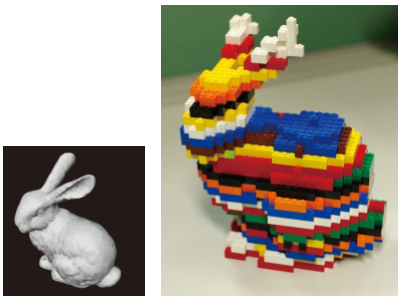
\includegraphics[width=0.5\textwidth]{BuiltLegoBunny}
  \caption{Actual buildings from produced manual given the model (Nakajima et al., 2013).}
\end{figure}

\begin{figure}[h!]
  \centering
  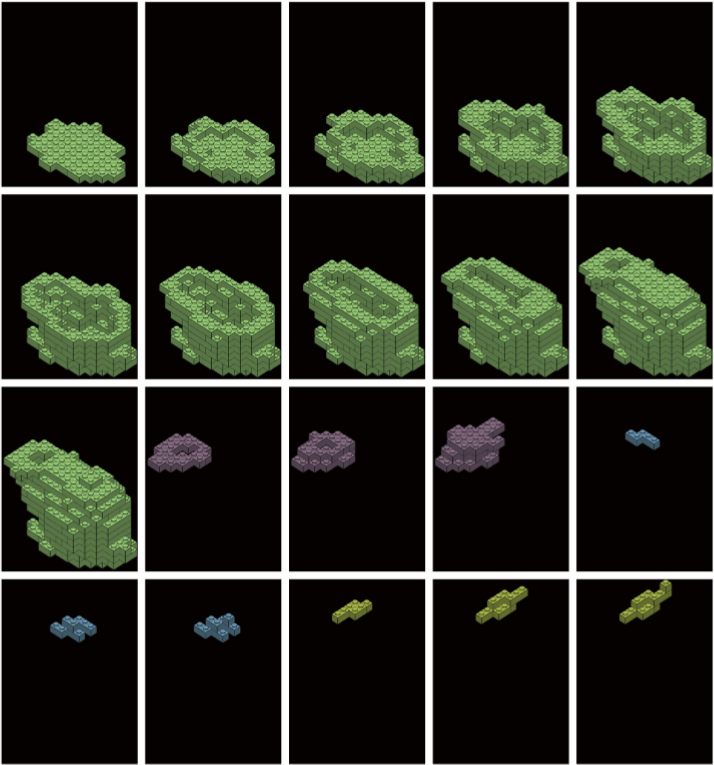
\includegraphics[width=0.5\textwidth]{AssemblyManualBunny}
  \caption{Assembly manual for the bunny model shown in Fig. 1.1 (Nakajima et al., 2013).
}
\end{figure}

% Define AR, common use/application, 
Augmented reality (AR) is a medium in which information are added and\slash or modified into the real physical world, usually through devices like AR glasses \cite{Craig20131}. Some of the common fields\slash areas where AR is applied are games, entertainment, medicine, and many more. A research by Pathomaree et al. extends its use on the manufacturing industry where manual and semi-automated labor is required \cite{Wang2016406}. Manufacturing was made more optimal by AR through using an enhanced bare-hand interface (EBHI) between the user and the system. The system of Pathomaree et al. was designed to be a guiding tool that helped users assemble objects and structures. Its implementation involved using a camera and augmented reality concepts to compute the interaction and hand gestures made by the user, which represented specific types of commands on navigating through the steps of the assembly of the object. Despite the feasibility and effectiveness of the said AR assembly guidance system, the study recommends further enhancements to the system by making it able to adapt to different cognitive ways it could assess a person's progress and enhancing its method of interaction with the user\slash s work.

\section{Research Objectives}
\label{sec:researchobjectives}

\subsection{General Objective}
\label{sec:generalobjective}

To design and develop a mobile application that serves as a tool that guides the user to build a LEGO structure, given a set of 3D voxel models of the stages of its construction as an input.


\subsection{Specific Objectives}
\label{sec:specificobjectives}

\begin{enumerate}
   \item To collate and review academic papers that discuss the applications of augmented reality and assembly guidance systems for manufacturing modeled objects.
	\item To design and develop a mobile application that uses augmented reality as its means of showing the next step a user should do to complete the assembly of the said structure.
	\item To analyze the mobile application's effectiveness in guiding the LEGO assembly by using the application to actually build the model and evaluating the process using evaluation metrics.
\end{enumerate}


\section{Scope and Limitations of the Research}
\label{sec:scopelimitations}

The research will focus on the assembly guidance mobile application for building LEGO models only. The system will not be used for assembling other objects. The research also does not include the transformation of LEGO 3D models into a set of instructions, as the assumed input is already the series of steps to assemble the 3D model.

Being designed and developed for a mobile phone, the research will only focus on using the mobile phone's camera for implementing the application itself. The research will also focus on dealing with blocks of the same height in order to simplify the research problem.

The developed mobile application will be subjected to usability testing as well as testing its comparison to other methods of assembling a LEGO model. The research does not analyze the structural strength of the resulting actual model.

%
%This section discusses the boundaries (with respect to the objectives) of the research and the constraints within 
%which the research will be developed.

\begin{comment}

%
% IPR acknowledgement: the sentences inside this comment are from Ethel Ong's slides on Scope and Limitations of the Research
%
Generally, one paragraph should be allotted for each of your research objectives.

Each paragraph contains a brief overview of the concept/theory and the purpose of doing the associated objective.

Each paragraph also includes a description of the scope/limitation of your study.

* Please refer to the slides for examples.

\end{comment}


\section{Significance of the Research}
\label{sec:significance}

\label{sec:significance}
This application can be used to aid LEGO designers, certified professionals and master builders cognitively in the construction of intricate LEGO models. In an experiment conducted by Curtin University, it was revealed the an animated AR system yielded shorter task completion times, less assembly errors, and lower total task load\cite{HouWangBernold2013}. 
The time that it takes to construct large LEGO models could also be drastically reduced with the use of this application. 

This application also has the potential to help teams of LEGO builders reduce the time that it takes to construct large LEGO models that would normally take days to complete.

This will also be beneficial to those who work in fields that take advantage of fast prototyping such as mechanical engineering, and fields that require the use of intricate structural prototypes such as architecture.

\begin{comment}
If applicable, describe possible commercialization and/or innovation in your research.
\end{comment}


